\subsection{Test results}
\label{subsec:test-res}

In this Section, we will analyze the performance of the submitted runs on heldout, short term and long term collections. At first, we will tackle the performance changes and then we will perform a \emph{statistical analysis}. In this last part, we will use ANOVA2 with a significance level $\alpha=0.05$ in order to find out if we can reject the \emph{null hypothesis}, i.e. there is no significant statistical difference between the results of the given runs. \\Then we will use Tukey's \ac{HSD} test to perform \emph{multiple} pairwise comparisons and determine which specific run means differ significantly from each other.

Since we have submitted four runs performed on the French collection and one on the English collection, in the statistical analysis we will compare to each other only the French runs.

\subsubsection{Heldout}
\label{subsubsec:heldout-res}

In Table~\ref{tab:heldout-map-ndcg-table} are reported the \ac{nDCG} and \ac{MAP} values obtained from the submitted runs on the heldout collection, while in Figure~\ref{fig:precision-recall-curve-heldout} is reported the interpolated Precision-Recall curve. Comparing these results with the ones obtained on training, shown in Table~\ref{tab:map-ndcg-table} and Figure~\ref{fig:precision-recall-curve} respectively, we can see that every run suffered a \emph{performance drop} over all the measures. This worsening was \emph{expected} and it can be due to the fact that the system has been tuned over a different set of queries. It should also be noticed that this set of queries is more than 6 times smaller compared to the training one, therefore the presence of some \emph{outliers} could have caused the mean performances to drop and to not be a good descriptor of the system.

Observing the \ac{nDCG} and \ac{AP} boxplots, shown in Figure~\ref{fig:heldout-boxplot}, we can notice that the runs performed on the French collection have a similar structure in terms of median values and interquartile ranges. We can also notice that, in the \ac{AP} boxplot, the reranked runs fr\_1, fr\_2 have longer whiskers, while the others show the presence of outliers.

From the ANOVA2 analysis, which results are reported in Table~\ref{tab:heldout-anova2}, we can see that $p\textrm{--}value>\alpha$, therefore we \emph{cannot reject} the null hypothesis. Moreover, from Tukey's \ac{HSD} multiple comparison shown in Figure~\ref{fig:heldout-hsd}, we can derive that the French runs can be considered to be similar to each other.

\begin{table}[tbp]
\caption{\ac{nDCG} and \ac{MAP} values on heldout collection}
  \label{tab:heldout-map-ndcg-table}
    \centering
    \begin{tabular}{|p{0.7\linewidth}|p{0.075\linewidth}|p{0.075\linewidth}|}
	\toprule
	\textbf{Run name} & \textbf{nDCG} & \textbf{MAP} \\
	\midrule
        FADERIC\_French-BM25-Stop50-LightStem-Shingle-Fuzzy-SynCustom-Rerank20W6 & 0.4169 & 0.2474 \\
        FADERIC\_French-BM25-Stop50-LightStem-Shingle-Fuzzy-Rerank30 & 0.4147 & 0.2416 \\
        FADERIC\_French-BM25-Stop50-LightStem-Shingle-Fuzzy-SynCustom & 0.4080 & 0.2376 \\
        FADERIC\_French-BM25Tuned-Stop50-LightStem-Shingle-Fuzzy & 0.4044 & 0.2324 \\
        FADERIC\_English-BM25-Stop50-KStem-Shingle-Fuzzy-SynPOS\\-Rerank30 & 0.3030 & 0.1626 \\
	\bottomrule
    \end{tabular}
\end{table}

\begin{figure}[tbp]
  \centering
  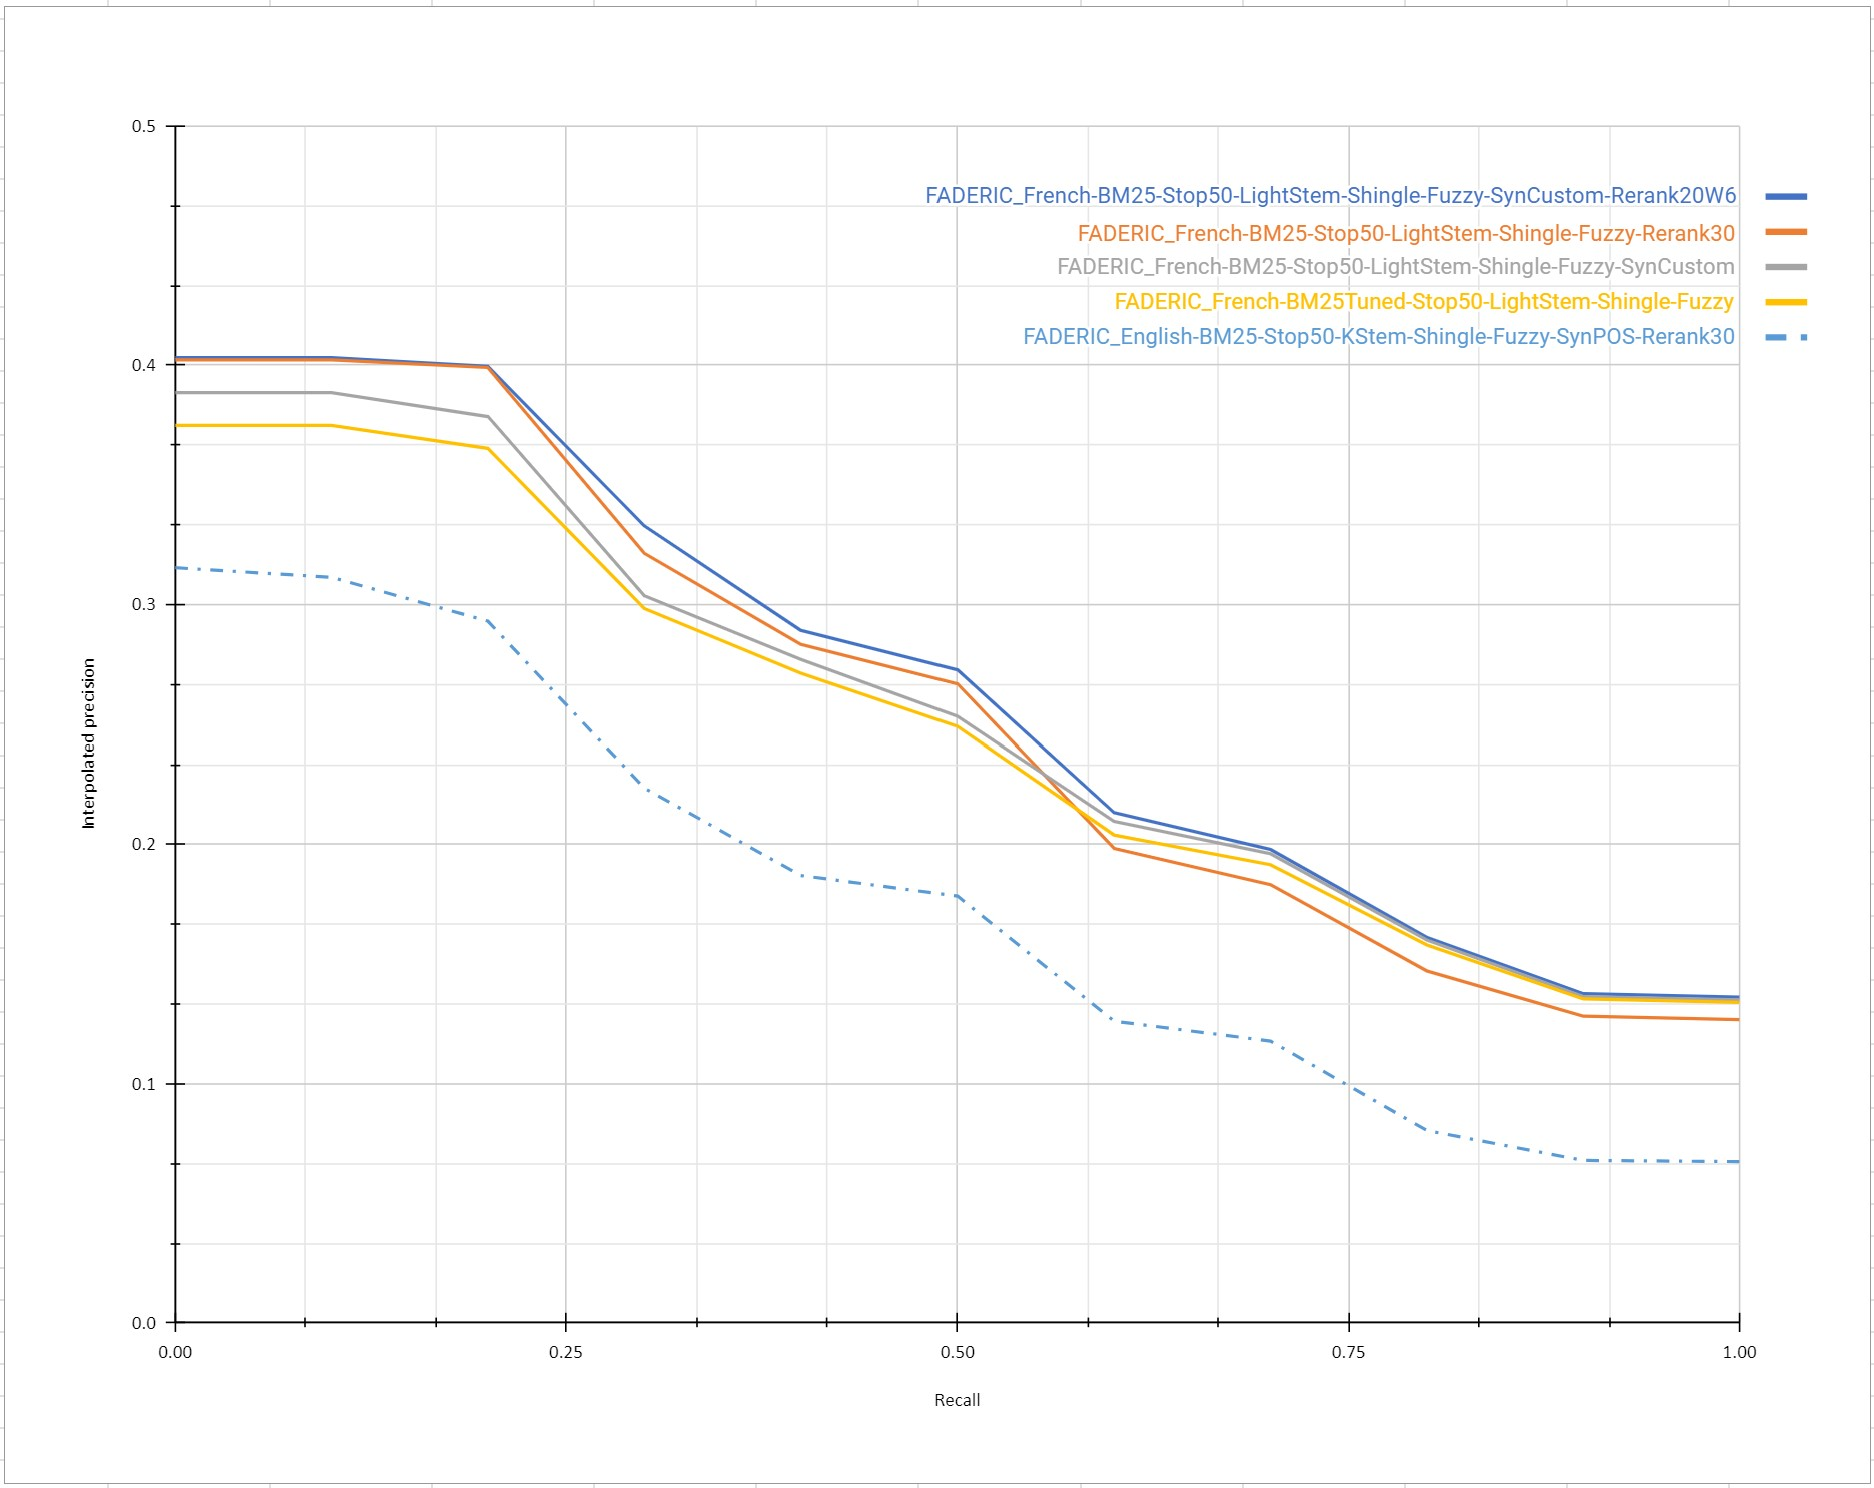
\includegraphics[width=1\linewidth]{figure/iprec-recall-HELDOUT.jpg}
  \caption{Interpolated Precision-Recall curve on heldout collection}
  \label{fig:precision-recall-curve-heldout}
\end{figure}

\begin{figure}[tbp]
     \centering
     \begin{subfigure}[b]{0.45\textwidth}
         \centering
         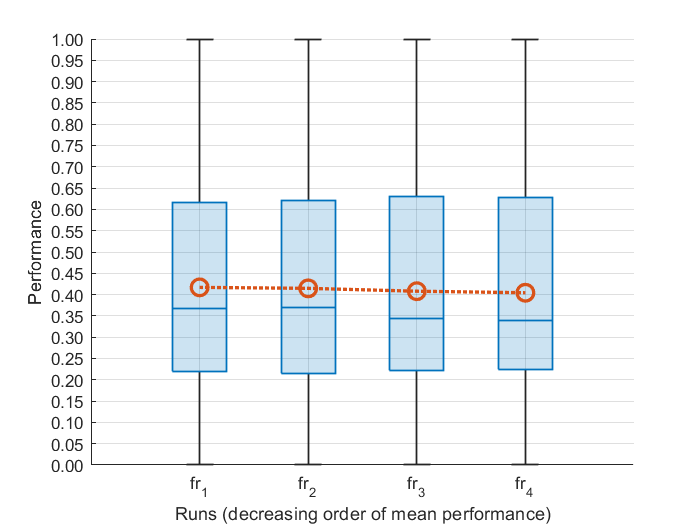
\includegraphics[width=\textwidth]{figure/heldout-ndcg-boxplot.png}
         \caption{\ac{nDCG}}
     \end{subfigure}
     \hfill
     \begin{subfigure}[b]{0.45\textwidth}
         \centering
         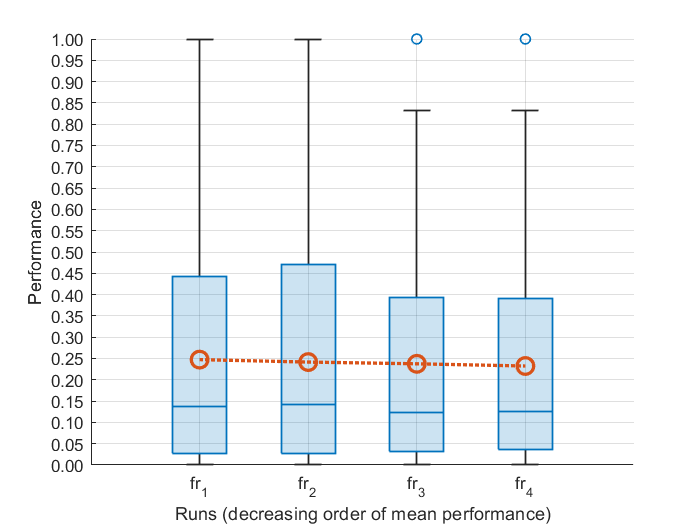
\includegraphics[width=\textwidth]{figure/heldout-map-boxplot.png}
         \caption{\ac{AP}}
     \end{subfigure}
        \caption{Box plot on heldout collection, the mean values are shown in red}
        \label{fig:heldout-boxplot}
\end{figure}

\begin{table}[tbp]
     \caption{ANOVA2 on heldout collection}
    \begin{subtable}[t]{1\textwidth}
        \centering
	\caption{\ac{nDCG}}
	\begin{tabular}{|l|l|l|l|l|l|}
	\toprule
        \textbf{Source} & \textbf{SS} & \textbf{df} & \textbf{MS} & \textbf{F} & \textbf{Prob$>$F} \\
        \midrule
	\textbf{Systems} & 0.01 & 3   & 0.003  & 0.64  & 0.58 \\
	\textbf{Topics}    & 23.54  & 97  & 0.242 & 47.20 & 1.97E-134 \\
	\textbf{Error}   & 1.49  & 291 & 0.005 & - & - \\
	\textbf{Total}   & 25.04  & 391 & - & - & - \\
	\bottomrule
       \end{tabular}
    \end{subtable}
        \begin{subtable}[t]{1\textwidth}
        \centering
	\caption{\ac{AP}}
        \begin{tabular}{|l|l|l|l|l|l|}
	\toprule
        \textbf{Source} & \textbf{SS} & \textbf{df} & \textbf{MS} & \textbf{F} & \textbf{Prob$>$F} \\
        \midrule
	\textbf{Systems} & 0.01 & 3  & 0.003  & 0.68  & 0.55 \\
	\textbf{Topics}    & 23.35  & 97  & 0.240 & 42.10 & 8.26E-128 \\
	\textbf{Error}   & 1.66  & 291 & 0.057 & - & - \\
	\textbf{Total}   & 25.03  & 391 & - & - & - \\
	\bottomrule
       \end{tabular}
    \end{subtable}
     \label{tab:heldout-anova2}
\end{table}

\begin{figure}[tbp]
     \centering
     \begin{subfigure}[b]{0.45\textwidth}
         \centering
         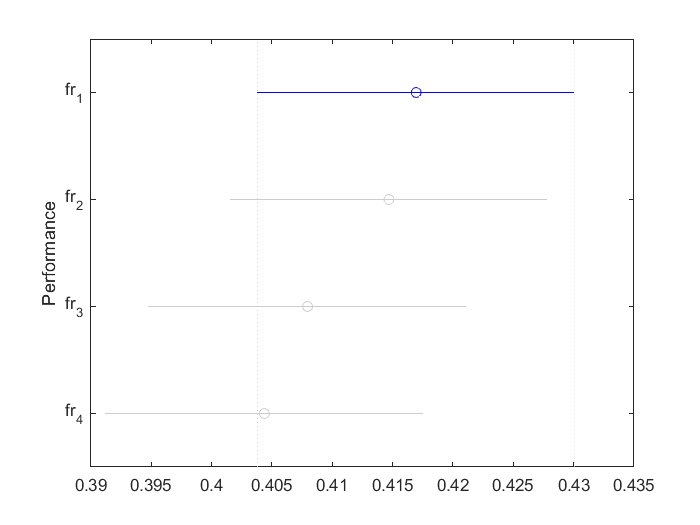
\includegraphics[width=\textwidth]{figure/heldout-ndcg-hsd.png}
	\caption{\ac{nDCG}}
     \end{subfigure}
     \hfill
     \begin{subfigure}[b]{0.45\textwidth}
         \centering
         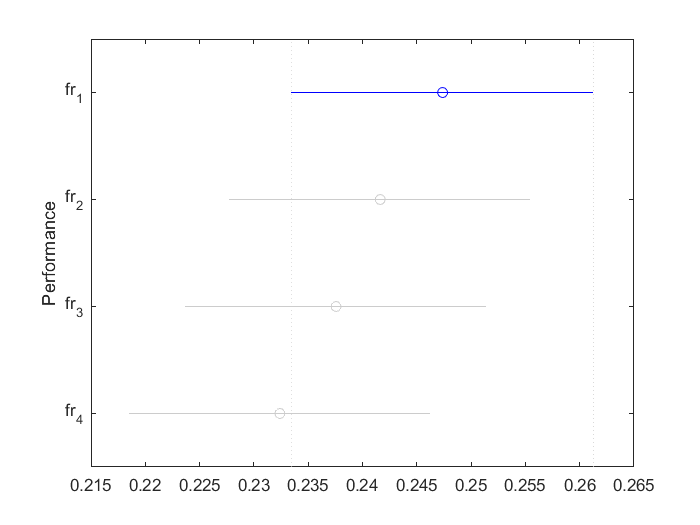
\includegraphics[width=\textwidth]{figure/heldout-map-hsd.png}
	\caption{\ac{AP}}
     \end{subfigure}
        \caption{Tukey's \ac{HSD} on heldout collection}
        \label{fig:heldout-hsd}
\end{figure}

\subsubsection{Short term}
\label{subsubsec:short-res}

In Table~\ref{tab:short-map-ndcg-table} are reported the \ac{nDCG} and \ac{MAP} values obtained from the submitted runs on the short term collection, while in Figure~\ref{fig:precision-recall-curve-short-term} is reported the interpolated Precision-Recall curve. Comparing these results with the ones obtained on heldout, shown in Table~\ref{tab:heldout-map-ndcg-table} and Figure~\ref{fig:precision-recall-curve-heldout} respectively, we can see that every run has \emph{increased} its performances. This improvement was \emph{not expected} since the performances should tend to drop over time. This can be due to the fact that this set of runs is almost 9 times bigger than the heldout, therefore we can consider the mean measures obtained to be more \emph{reliable} than the ones on the heldout collection.

Observing the \ac{nDCG} and \ac{AP} boxplots, shown in Figure~\ref{fig:short-boxplot}, we can notice that the runs performed on the French collection have a similar structure in terms of median values and interquartile ranges. We can also notice that in the \ac{AP} boxplot the fr\_1 run has a longer whisker, while the others show the presence of outliers.

From the ANOVA2 analysis, which results are reported in Table~\ref{tab:short-anova2}, we can see that $p\textrm{--}value<\alpha$, therefore we \emph{can reject} the null hypothesis. Moreover, from Tukey's \ac{HSD} multiple comparison shown in Figure~\ref{fig:short-hsd}, we can derive that runs fr\_3, fr\_4 can be considered similar, while all the other runs differ from each other.

\begin{table}[tbp]
\caption{\ac{nDCG} and \ac{MAP} values on short term collection}
  \label{tab:short-map-ndcg-table}
    \centering
    \begin{tabular}{|p{0.7\linewidth}|p{0.075\linewidth}|p{0.075\linewidth}|}
	\toprule
	\textbf{Run name} & \textbf{nDCG} & \textbf{MAP} \\
	\midrule
        FADERIC\_French-BM25-Stop50-LightStem-Shingle-Fuzzy-SynCustom-Rerank20W6 & 0.4239 & 0.2665 \\ 
        FADERIC\_French-BM25-Stop50-LightStem-Shingle-Fuzzy-Rerank30 & 0.4145 & 0.2546 \\ 
        FADERIC\_French-BM25-Stop50-LightStem-Shingle-Fuzzy-SynCustom & 0.4034 & 0.2412 \\ 
        FADERIC\_French-BM25Tuned-Stop50-LightStem-Shingle-Fuzzy & 0.4034 & 0.2414 \\ 
        FADERIC\_English-BM25-Stop50-KStem-Shingle-Fuzzy-SynPOS\\-Rerank30 & 0.3296 & 0.1931 \\ 
	\bottomrule
    \end{tabular}
\end{table}

\begin{figure}[tbp]
  \centering
  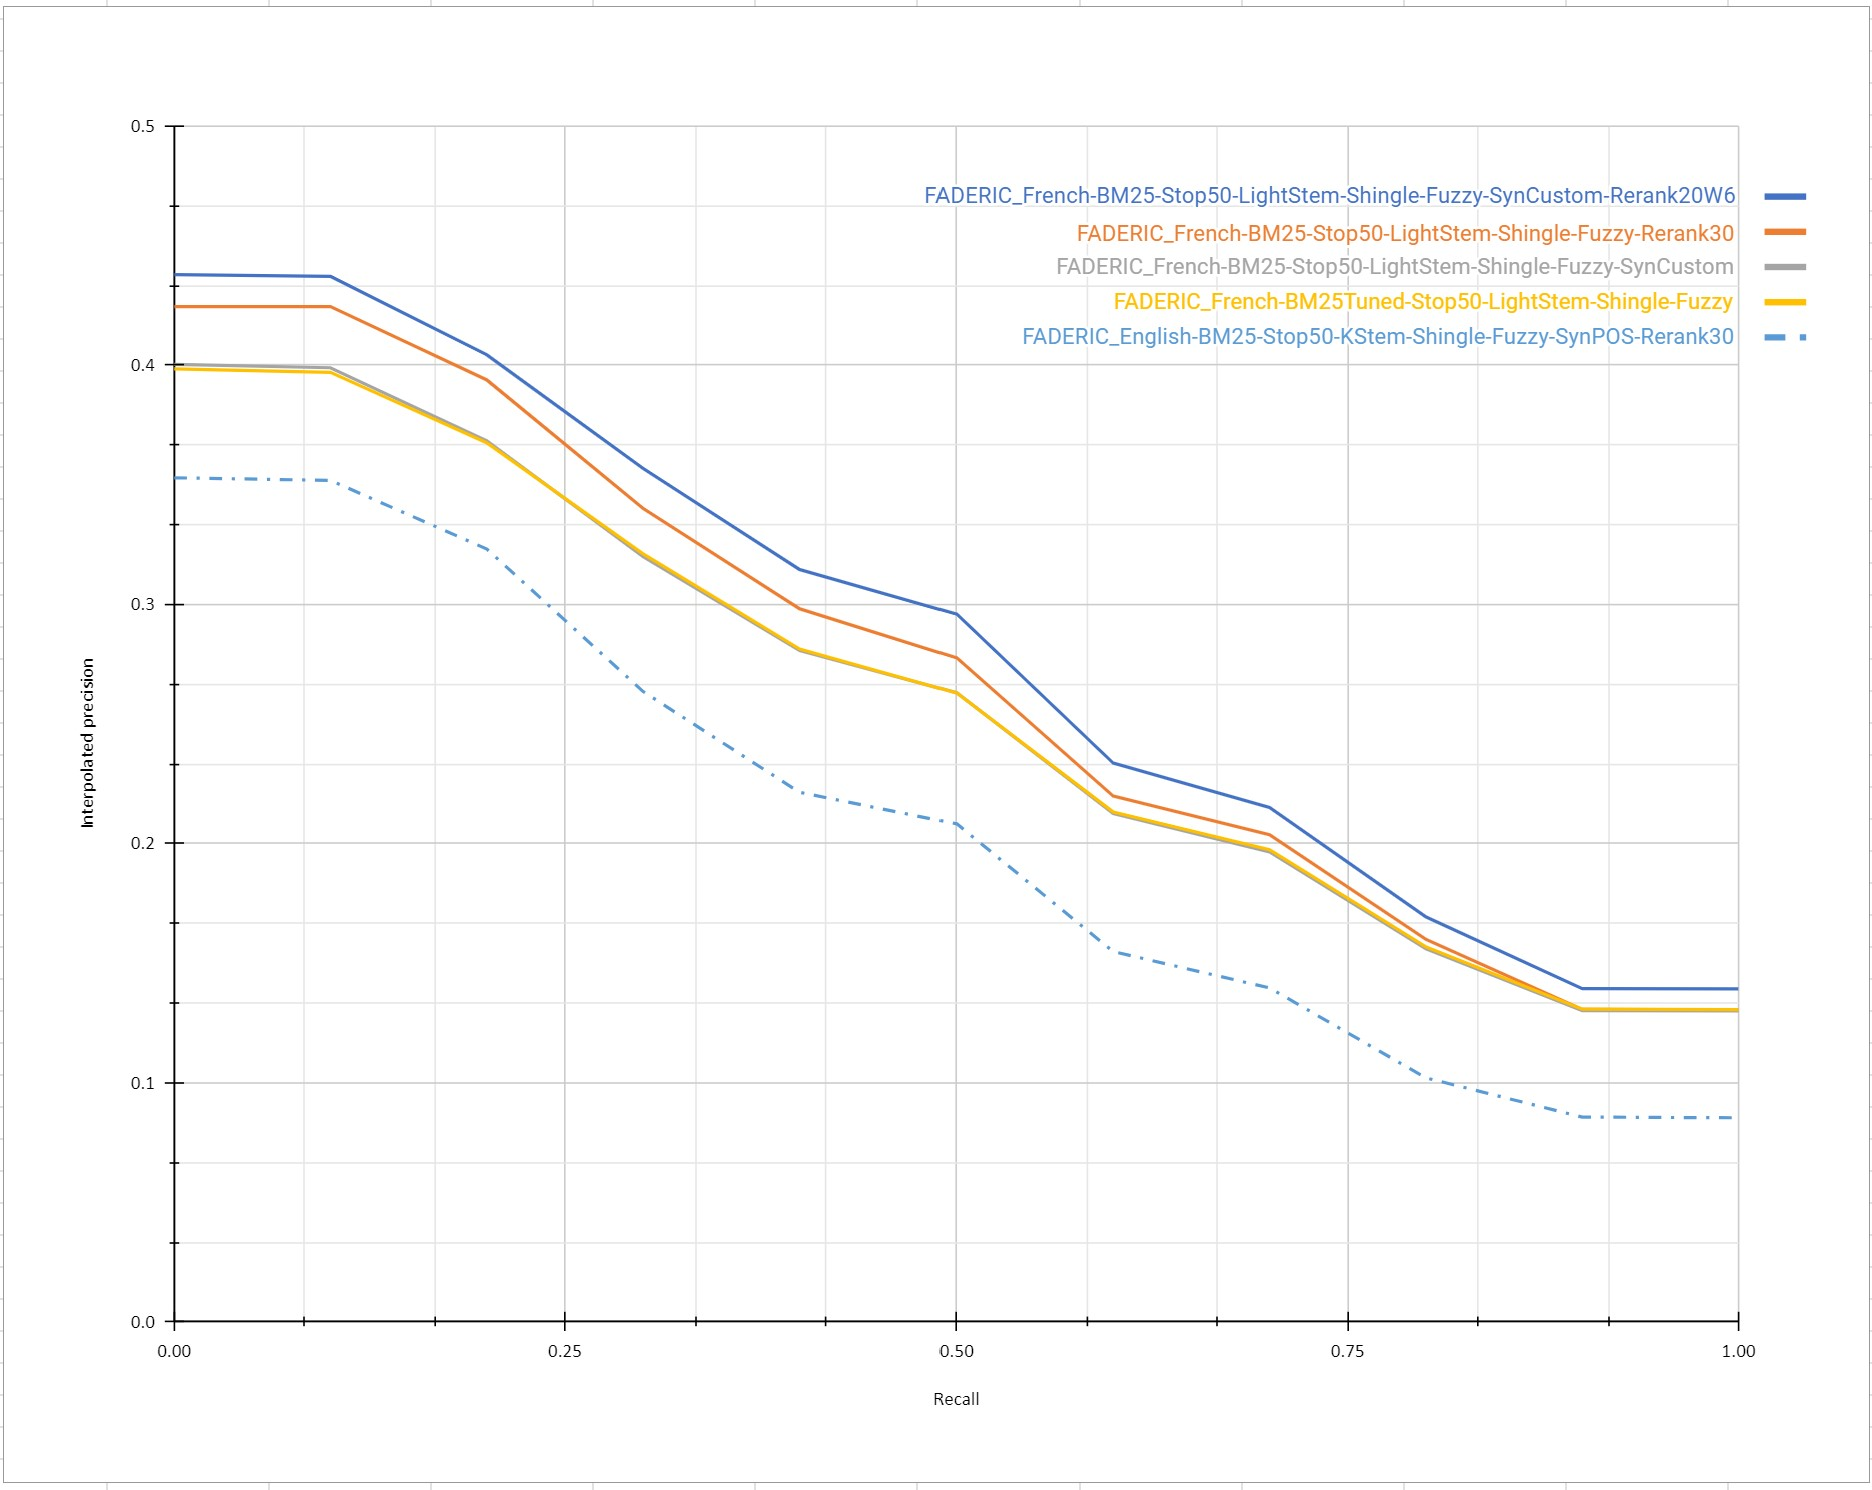
\includegraphics[width=1\linewidth]{figure/iprec-recall-SHORT-TERM.jpg}
  \caption{Interpolated Precision-Recall curve on short term collection}
  \label{fig:precision-recall-curve-short-term}
\end{figure}

\begin{figure}[tbp]
     \centering
     \begin{subfigure}[b]{0.45\textwidth}
         \centering
         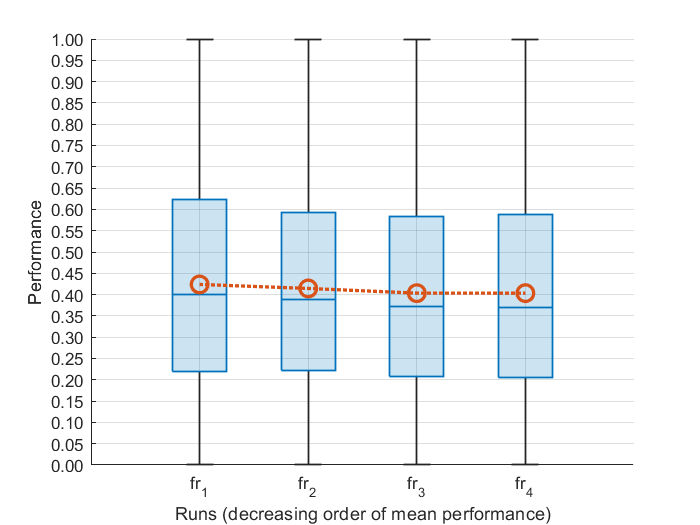
\includegraphics[width=\textwidth]{figure/short-ndcg-boxplot.png}
         \caption{\ac{nDCG}}
     \end{subfigure}
     \hfill
     \begin{subfigure}[b]{0.45\textwidth}
         \centering
         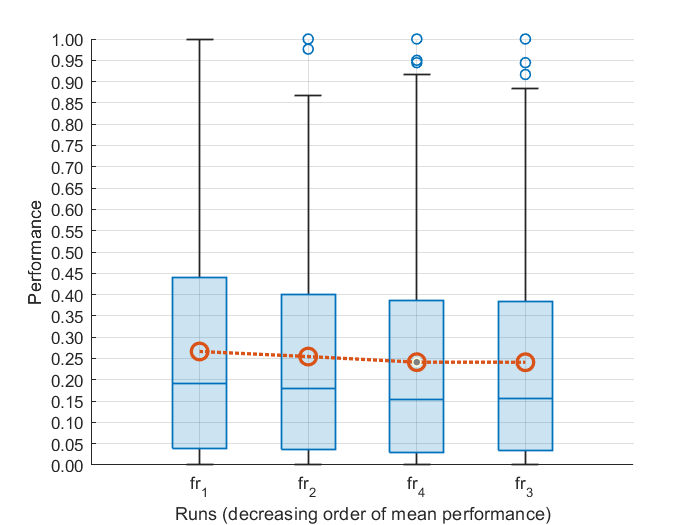
\includegraphics[width=\textwidth]{figure/short-map-boxplot.png}
         \caption{\ac{AP}}
     \end{subfigure}
        \caption{Box plot on short term collection, the mean values are shown in red}
        \label{fig:short-boxplot}
\end{figure}

\begin{table}[tbp]
     \caption{ANOVA2 on short term collection}
    \begin{subtable}[h]{1\textwidth}
        \centering
	 \caption{\ac{nDCG}}
        \begin{tabular}{|l|l|l|l|l|l|}
	\toprule
        \textbf{Source} & \textbf{SS} & \textbf{df} & \textbf{MS} & \textbf{F} & \textbf{Prob$>$F} \\
        \midrule
	\textbf{Systems} & 0.25 & 3  & 0.085  & 13.58  & 8.51E-9 \\
	\textbf{Topics}    & 218.58  & 881  & 0.248 & 39.30 & 0 \\
	\textbf{Error}   & 16.68 & 2643 & 0.006 & - & - \\
	\textbf{Total}   & 235.52  & 3527 & - & - & - \\
	\bottomrule
       \end{tabular}
    \end{subtable}
        \begin{subtable}[h]{1\textwidth}
        \centering
	\caption{\ac{AP}}
        \begin{tabular}{|l|l|l|l|l|l|}
	\toprule
        \textbf{Source} & \textbf{SS} & \textbf{df} & \textbf{MS} & \textbf{F} & \textbf{Prob$>$F} \\
        \midrule
	\textbf{Systems} & 0.38 & 3   & 0.129  & 16.05  & 2.43E-10 \\
	\textbf{Topics}    & 205.64  & 881  & 0.233 & 28.92 & 0 \\
	\textbf{Error}   & 21.32  & 2643 & 0.008 & - & - \\
	\textbf{Total}   & 227.36  & 3527 & - & - & - \\
	\bottomrule
       \end{tabular}
    \end{subtable}
     \label{tab:short-anova2}
\end{table}

\begin{figure}[tbp]
     \centering
     \begin{subfigure}[b]{0.45\textwidth}
         \centering
         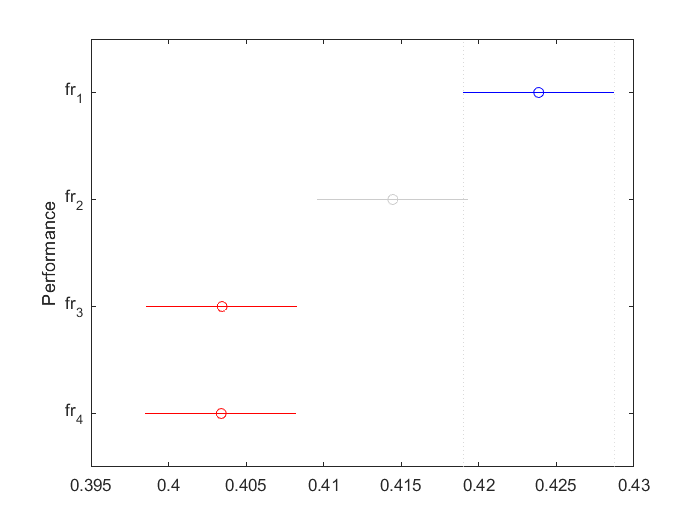
\includegraphics[width=\textwidth]{figure/short-ndcg-hsd.png}
	\caption{\ac{nDCG}}
     \end{subfigure}
     \hfill
     \begin{subfigure}[b]{0.45\textwidth}
         \centering
         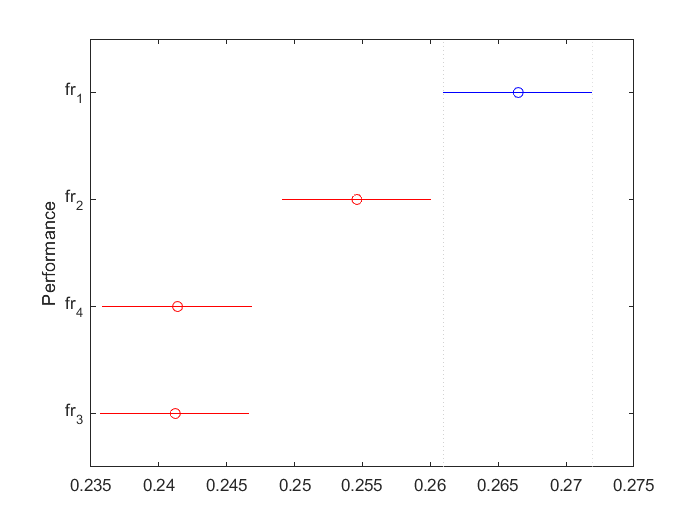
\includegraphics[width=\textwidth]{figure/short-map-hsd.png}
	\caption{\ac{AP}}
     \end{subfigure}
        \caption{Tukey's \ac{HSD} on short term collection}
        \label{fig:short-hsd}
\end{figure}

\clearpage

\subsubsection{Long term}
\label{subsubsec:long-res}

Since some error occurred in the indexing phase when performing the submitted runs fr\_1 and fr\_2, in the following analysis we will use a \emph{fixed} version of those runs.

In Table~\ref{tab:long-map-ndcg-table} are reported the \ac{nDCG} and \ac{MAP} values obtained from the submitted runs on the long term collection, while in Figure~\ref{fig:precision-recall-curve-long-term} is reported the interpolated Precision-Recall curve. Comparing these results with the ones obtained on the short term, shown in Table~\ref{tab:short-map-ndcg-table} and Figure~\ref{fig:precision-recall-curve-short-term} respectively, we can see that every run suffered a \emph{performance drop} over all the measures. This worsening was expected and it can be due to the fact that the performances tend to drop over time, however, the decrease is not huge and we can consider the performances of the system to \emph{remain satisfactory}.

Observing the \ac{nDCG} and \ac{AP} boxplots, shown in Figure~\ref{fig:long-boxplot}, we can notice that the runs performed on the French collection have a similar structure in terms of median values and interquartile ranges. We can also notice that in the \ac{AP} boxplot all the runs show the presence of outliers. 

From the ANOVA2 analysis, which results are reported in Table~\ref{tab:long-anova2}, we can see that we obtained very different results for the two measures. In particular, on \ac{nDCG} we have $p\textrm{--}value>\alpha$, which means we \emph{cannot reject} the null hypothesis, while on \ac{AP} we have $p\textrm{--}value<\alpha$, which means we \emph{can reject} the null hypothesis. The same behavior is reflected in Tukey's \ac{HSD} multiple comparison, shown in Figure~\ref{fig:long-hsd}, where on \ac{nDCG} we can derive that the French runs can be considered to be similar to each other, while on \ac{AP}  we can see that runs fr\_1, fr\_2, fr\_3 and runs fr\_3, fr\_4 can be considered similar to each other.

\begin{table}[tbp]
\caption{\ac{nDCG} and \ac{MAP} values on long term collection}
  \label{tab:long-map-ndcg-table}
    \centering
    \begin{tabular}{|p{0.7\linewidth}|p{0.075\linewidth}|p{0.075\linewidth}|}
	\toprule
	\textbf{Run name} & \textbf{nDCG} & \textbf{MAP} \\
	\midrule
        FADERIC\_French-BM25-Stop50-LightStem-Shingle-Fuzzy-SynCustom-Rerank20W6 & 0.4153 & 0.2473 \\ 
        FADERIC\_French-BM25-Stop50-LightStem-Shingle-Fuzzy-Rerank30 & 0.4146 & 0.2465 \\ 
        FADERIC\_French-BM25-Stop50-LightStem-Shingle-Fuzzy-SynCustom & 0.4091 & 0.2384 \\ 
        FADERIC\_French-BM25Tuned-Stop50-LightStem-Shingle-Fuzzy & 0.4071 & 0.2350 \\ 
        FADERIC\_English-BM25-Stop50-KStem-Shingle-Fuzzy-SynPOS\\-Rerank30 & 0.3296 & 0.1809 \\ 
	\bottomrule
    \end{tabular}
\end{table}

\begin{figure}[tbp]
  \centering
  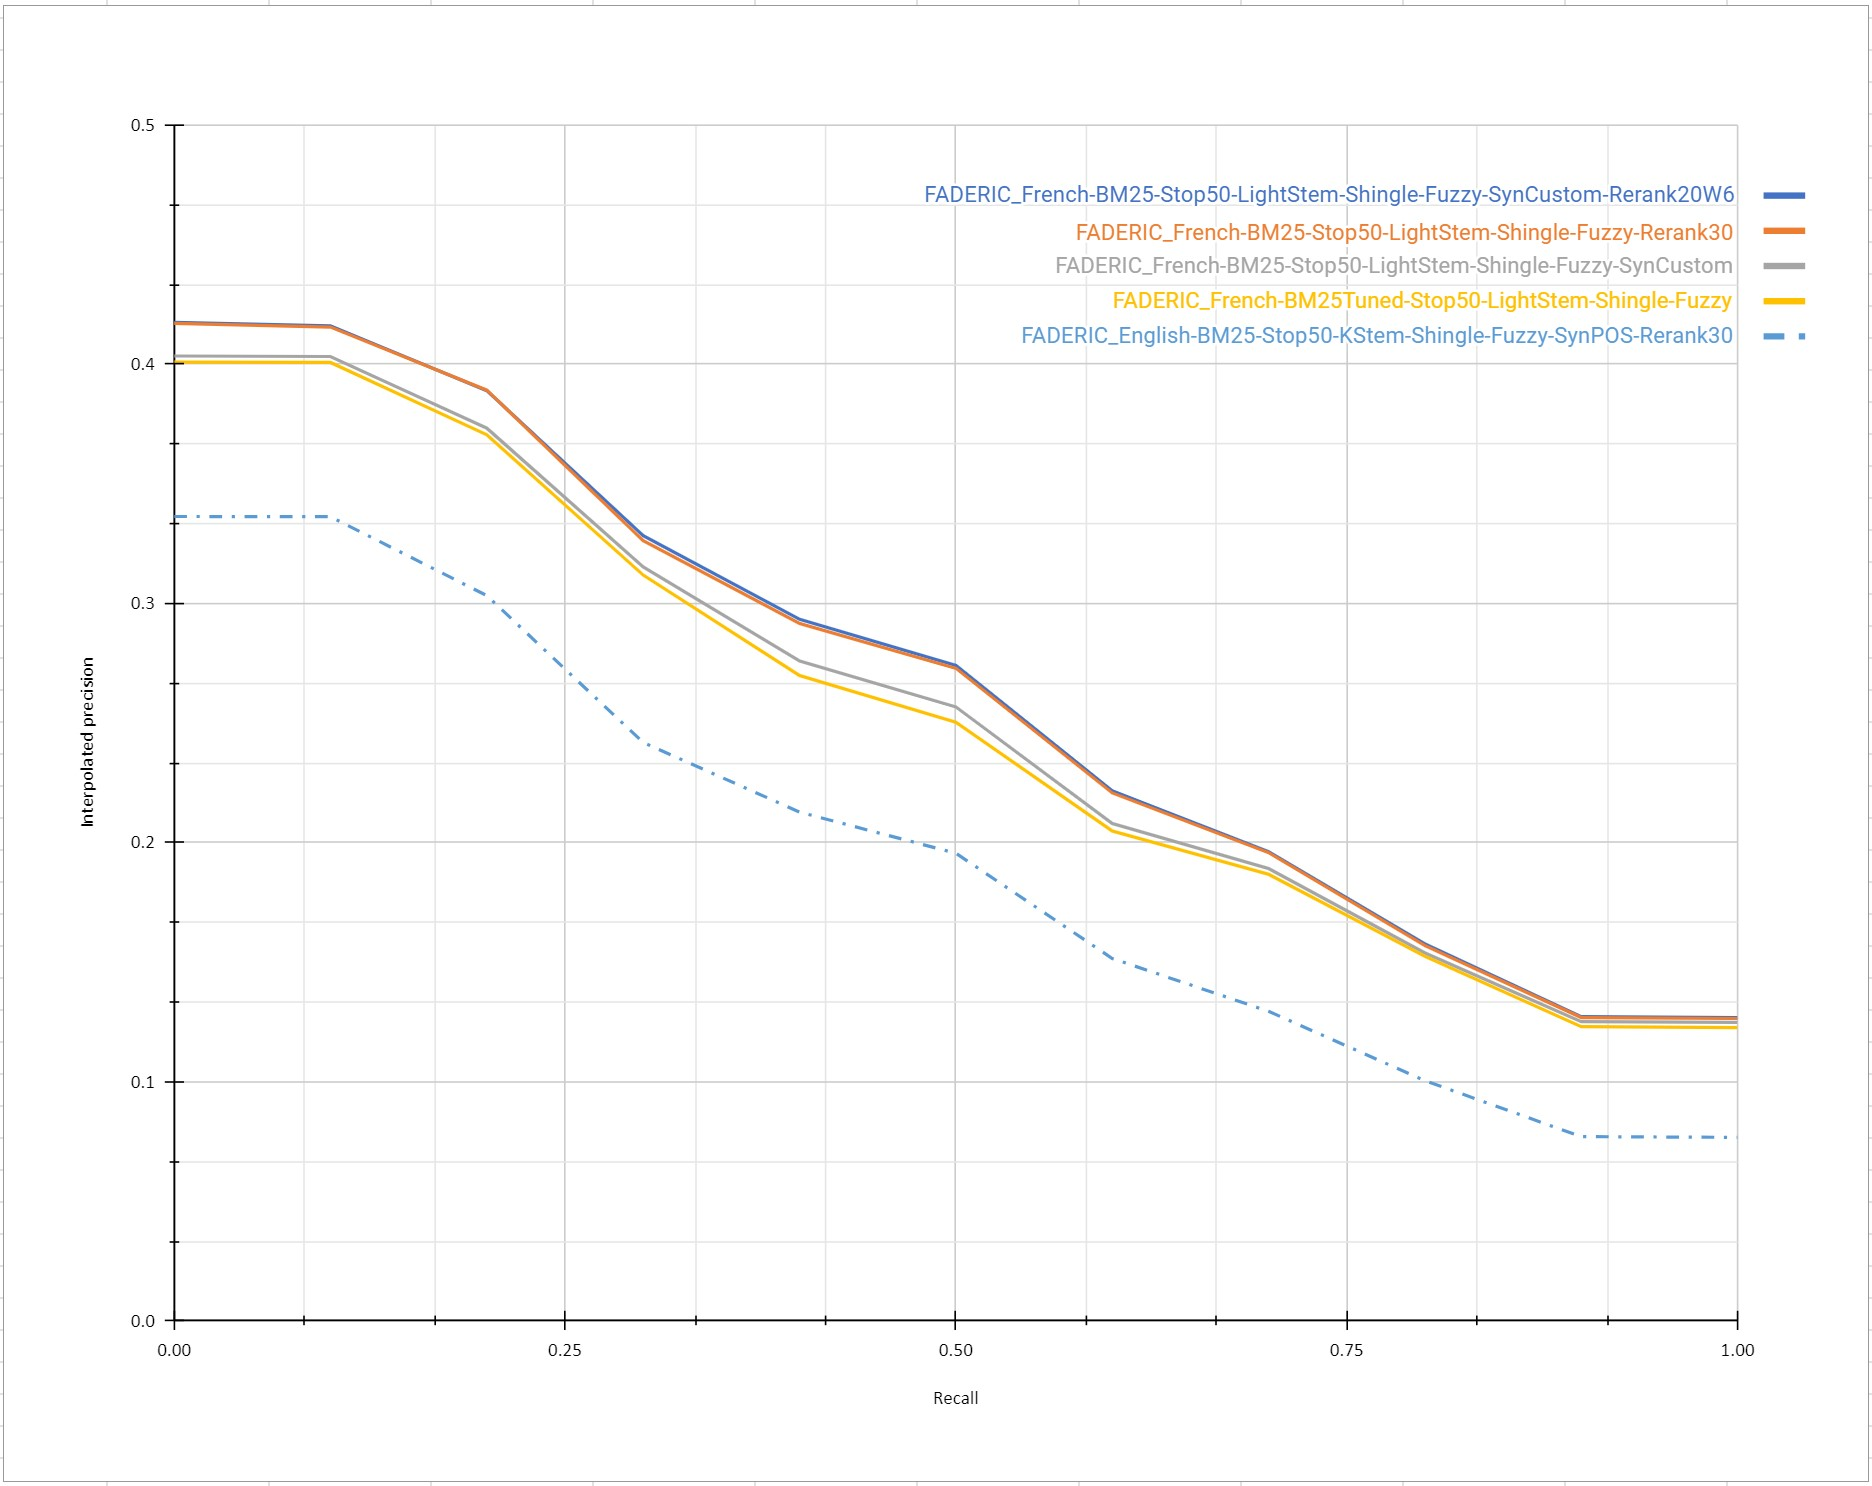
\includegraphics[width=1\linewidth]{figure/iprec-recall-LONG-TERM.jpg}
  \caption{Interpolated Precision-Recall curve on long term collection}
  \label{fig:precision-recall-curve-long-term}
\end{figure}

\begin{figure}[tbp]
     \centering
     \begin{subfigure}[b]{0.45\textwidth}
         \centering
         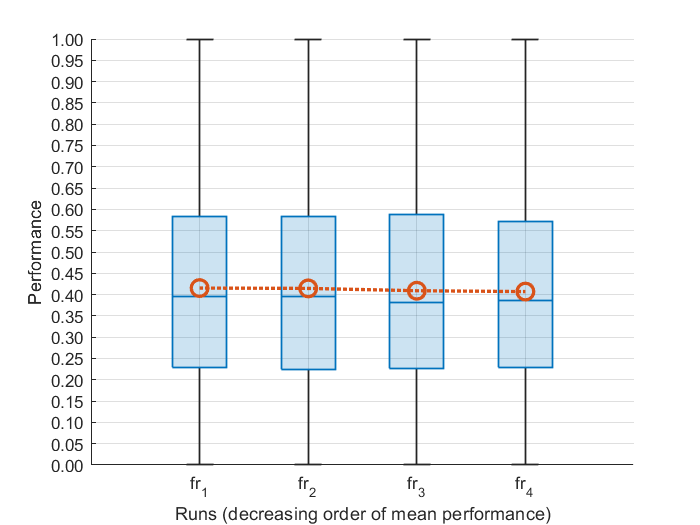
\includegraphics[width=\textwidth]{figure/long-ndcg-boxplot.png}
         \caption{\ac{nDCG}}
     \end{subfigure}
     \hfill
     \begin{subfigure}[b]{0.45\textwidth}
         \centering
         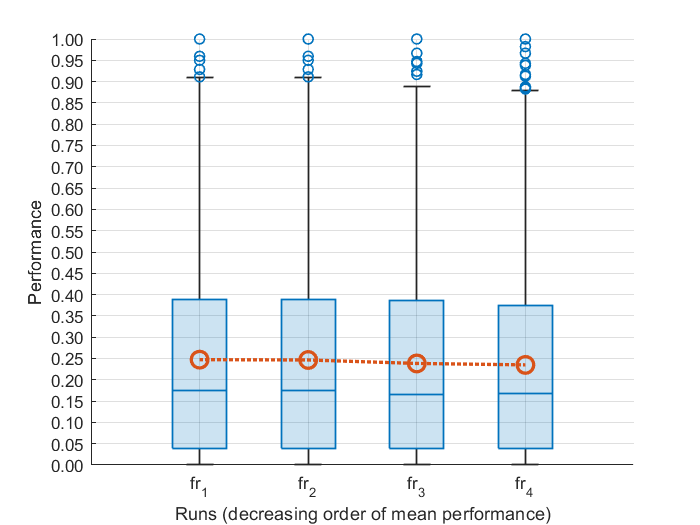
\includegraphics[width=\textwidth]{figure/long-map-boxplot.png}
         \caption{\ac{AP}}
     \end{subfigure}
        \caption{Box plot on long term collection, the mean values are shown in red}
        \label{fig:long-boxplot}
\end{figure}

\begin{table}[tbp]
     \caption{ANOVA2 on long term collection}
    \begin{subtable}[h]{1\textwidth}
        \centering
	\caption{\ac{nDCG}}
        \begin{tabular}{|l|l|l|l|l|l|}
	\toprule
        \textbf{Source} & \textbf{SS} & \textbf{df} & \textbf{MS} & \textbf{F} & \textbf{Prob$>$F} \\
        \midrule
	\textbf{Systems} & 0.04 & 3   & 0.015  & 1.51  & 0.056 \\
	\textbf{Topics}    & 202.35  & 922  & 0.219 & 16.17 & 0 \\
	\textbf{Error}   & 16.78  & 2766 & 0.006 & - & - \\
	\textbf{Total}   & 219.18  & 3691 & - & - & - \\
	\bottomrule
       \end{tabular}
    \end{subtable}
        \begin{subtable}[h]{1\textwidth}
        \centering
	\caption{\ac{AP}}
        \begin{tabular}{|l|l|l|l|l|l|}
	\toprule
        \textbf{Source} & \textbf{SS} & \textbf{df} & \textbf{MS} & \textbf{F} & \textbf{Prob$>$F} \\
        \midrule
	\textbf{Systems} & 0.10 & 3   & 0.033  & 4.47  & 0.003 \\
	\textbf{Topics}    & 188.61  & 922  & 0.204 & 27.03 & 0 \\
	\textbf{Error}   & 20.92  & 2766 & 0.007 & - & - \\
	\textbf{Total}   & 209.64  & 3691 & - & - & - \\
	\bottomrule
       \end{tabular}
    \end{subtable}
     \label{tab:long-anova2}
\end{table}

\begin{figure}[tbp]
     \centering
     \begin{subfigure}[b]{0.4\textwidth}
         \centering
         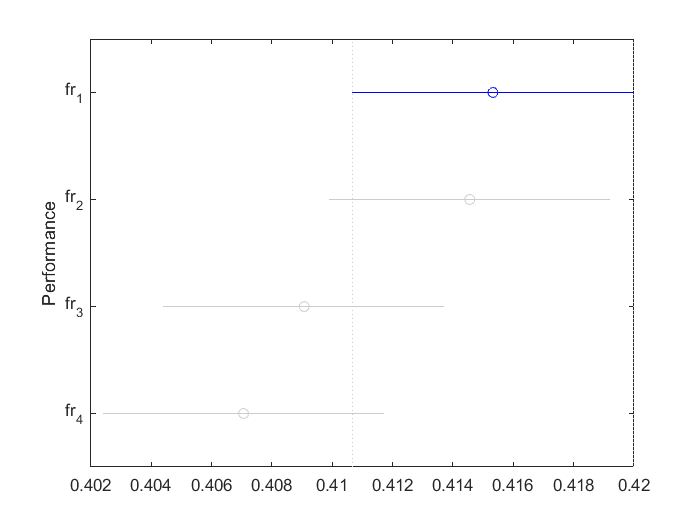
\includegraphics[width=\textwidth]{figure/long-ndcg-hsd.png}
	\caption{\ac{nDCG}}
     \end{subfigure}
     \hfill
     \begin{subfigure}[b]{0.4\textwidth}
         \centering
         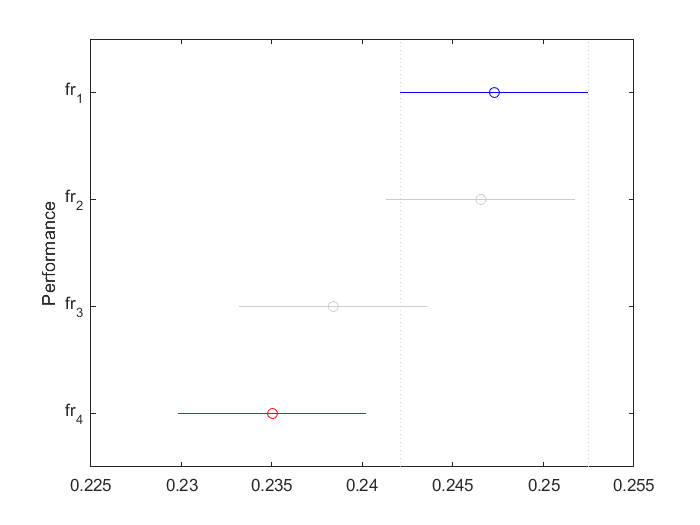
\includegraphics[width=\textwidth]{figure/long-map-hsd.png}
	\caption{\ac{AP}}
     \end{subfigure}
        \caption{Tukey's \ac{HSD} on long term collection}
        \label{fig:long-hsd}
\end{figure}